\documentclass{../../../oss-classkick-exam}
\usepackage{wrapfig}

\begin{document}
\genheader

\gentitle{C}{WORK AND ENERGY}

\genmultidirections

\gengravity

\raggedcolumns
\begin{multicols*}{2}

  \begin{questions}

    \question A \SI1{\kilo\gram} ball is thrown vertically downward from a
    \SI{50}{\metre} high tower with an initial speed of \SI4{\metre\per\second}.
    Just before striking the ground, the speed of the ball is
    \SI{20}{\metre\per\second}. The energy lost to air friction is most nearly
    \begin{choices}
      \choice\SI{101}{\joule}
      \choice\SI{210}{\joule}
      \choice\SI{308}{\joule}
      \choice\SI{406}{\joule}
      \choice\SI{508}{\joule}
    \end{choices}

    \uplevel{
      \textbf{Questions \ref{q:pq1}--\ref{q:pq2}}\\
      A \SI2{\kilo\gram} projectile is launched with a speed of
      \SI{20}{\metre\per\second} from horizontal ground at an angle of \ang{37}
      to the horizontal as shown. Point $P$ is at the top of the path, and
      point $Q$ is at the end of the path, just before the projectile again
      reaches the ground.
      \cpic{.35}{symprojectile}
    }

  \item The kinetic energy of the projectile at point $P$ is
    \label{q:pq1}
    \begin{choices}
      \choice\SI{108}{\joule}
      \choice\SI{225}{\joule}
      \choice\SI{256}{\joule}
      \choice\SI{400}{\joule}
      \choice\SI{525}{\joule}
    \end{choices}
    
  \item The kinetic energy of the projectile at point $Q$ is
    \label{q:pq2}
    \begin{choices}
      \choice\SI{108}{\joule}
      \choice\SI{225}{\joule}
      \choice\SI{256}{\joule}
      \choice\SI{400}{\joule}
      \choice\SI{525}{\joule}
    \end{choices}
    
    \question If a projectile thrown directly upward reaches a maximum height
    $h$ and spends a total time in the air of $T$, then returning to the
    original location, the average power of the gravitational force during the
    trajectory is
    \begin{choices}
      \choice $P=2mgh/T$
      \choice $P=-2mgh/T$
      \choice 0
      \choice $P=mgh/T$
      \choice $P=-mgh/T$
    \end{choices}
    \vspace{.7in}
    
    \question Given that the constant net force on an object and the object's 
    displacement, which of the following quantities can be calculated?
    \begin{choices}
      \choice the net change in the object's velocity
      \choice the net change in the object's mechanical energy
      \choice the average acceleration
      \choice the net change in the object's kinetic energy
      \choice the net change in the object's potential energy
    \end{choices}
    \vspace{.7in}
    
    \question The force acting on an object varies with the equation
    $F(x)=-3x^2-2x-4$, where force is in newtons and displacement is in meters.
    The potential energy at $x=\SI2{\metre}$ is
    \begin{choices}
      \choice zero
      \choice\SI{20}{\joule}
      \choice\SI{40}{\joule}
      \choice\SI{-20}{\joule}
      \choice\SI{-40}{\joule}
    \end{choices}
    \columnbreak
    
    \question If the only force acting on an object is given by the equation
    $F(x)=2-4x$ (where the force is measured in newtons and position in meters),
    what is the change in the object's kinetic energy as it moves from $x=2$ to
    $x=1$?
    \begin{choices}
      \choice +\SI{4}{\joule}
      \choice \SI{-4}{\joule}
      \choice +\SI{2}{\joule}
      \choice \SI{-2}{\joule}
      \choice +\SI{8}{\joule}
    \end{choices}
    
    \question The potential energy of an object varies with the equation
    $U(x)=2x^2+x-6$, where force is in newtons and displacement is in meters. A
    force $F$ vs.\ displacement $x$ graph would yield which of the following?
    \begin{choices}
      \choice A straight, horizontal line
      \choice A parabola
      \choice An exponential decay curve
      \choice A straight line with a positive slope
      \choice A straight line with a negative slope
    \end{choices}
    \vspace{.7in}
    
    \question A particle of mass $m$ moves according to the displacement
    equation $x=2t^{5/2}$. The kinetic energy of the particle as a function of
    time is
    \begin{choices}
      \choice $10mt^{5/2}$
      \choice $10mt^{3/2}$
      \choice $\dfrac{25}2mt^3$
      \choice $5mt^2$
      \choice $2mt^{3/2}$
    \end{choices}

    \question An electron travels in a circle around a hydrogen nucleus at a
    very high speed. The work done by the electrostatic force acting on the
    electron after one complete revolution is
    \begin{choices}
      \choice zero
      \choice positive
      \choice negative
      \choice equal to the kinetic energy of the electron
      \choice equal to the potential energy of the electron
    \end{choices}
    \vspace{.7in}
    
    \question An object is moved from rest at point $P$ to rest at point $Q$ in
    a gravitational field. The net work against the gravitational field depends
    on the
    \begin{choices}
      \choice mass of the object and the positions of $P$ and $Q$
      \choice mass of the object only
      \choice positions of $P$ and $Q$ only
      \choice length moved between points $P$ and $Q$
      \choice coefficient of friction
    \end{choices}
    \columnbreak

    \uplevel{
      \textbf{Questions \ref{q:well1}--\ref{q:well2}}\\
      Consider the potential energy function shown below.
      \cpic{.28}{potential-well}
    }

    \question Assuming that no non-conservative forces are present, if a
    particle of mass $m$ is released from position $x_0$, what is the maximum
    speed it will achieve?
    \label{q:well1}
    \begin{choices}
      \choice $\sqrt{4U_0/m}$
      \choice $\sqrt{2U_0/m}$
      \choice $\sqrt{U_0/m}$
      \choice $\sqrt{U_0/2m}$
      \choice The particle will achieve no maximum speed but instead will
      continue to accelerate indefinitely.
    \end{choices}
    \vspace{.7in}
    
    \question Which of the following is the most accurate description of the
    system introduced in the previous question?
    \label{q:well2}
    \begin{choices}
      \choice A stable equilibrium
      \choice An unstable equilibrium
      \choice A neutral equilibrium
      \choice A bound system
      \choice There is a linear restoring force
    \end{choices}
    \vspace{.7in}
    
    \question A pendulum bob of mass $m$ is released from rest as shown in the
    figure below. What is the tension in the string as the pendulum swings
    through the lowest point of its motion?
    \begin{center}
      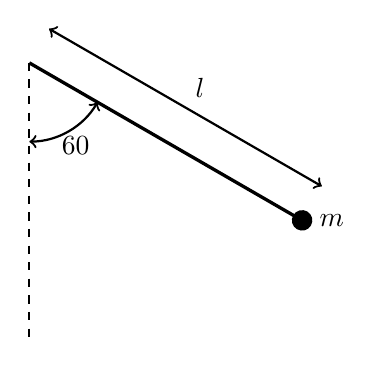
\begin{tikzpicture}
        \draw[thick,dashed](0,0)--(0,-3.5);
        \begin{scope}[rotate=60]
          \draw[very thick](0,0)--(0,-4);
          \fill(0,-4) circle(.13) node[right]{$\;m$};
          \draw[<->,thick](.5,0)--(.5,-4) node[midway,above right]{$l$};
        \end{scope}
        \draw[<->,thick](0,-1)arc(270:330:1)
        node[pos=.6,below]{\ang{60}};
      \end{tikzpicture}
    \end{center}
    \begin{choices}
      \choice $T=\dfrac12mg$
      \choice $T=mg$
      \choice $T=d\frac32mg$
      \choice $T=2mg$
      \choice None of the above
    \end{choices}
    
    \question Two blocks of mass $m_A$ and $m_B$ are connected by a string that
    passes over a light pulley. The mass of $A$ is larger than the mass of $B$.
    The speed of mass $A$ just before reaching the floor is:
    \begin{center}
      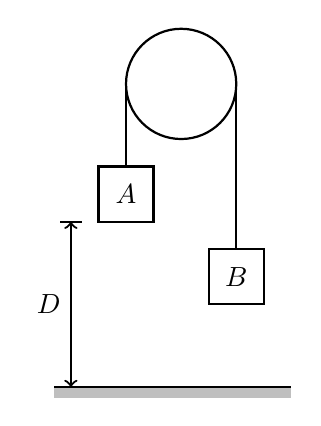
\begin{tikzpicture}[scale=.7]
        \begin{scope}[thick]
          \draw(0,0) circle(1);
          \draw(-1,0)--(-1,-1.5);
          \draw(-1.5,-1.5) rectangle(-.5,-2.5) node[midway]{$A$};
          \draw(1,0)--(1,-3);
          \draw(1.5,-3) rectangle(.5,-4)  node[midway]{$B$};
          \draw(-1.8,-2.5)--(-2.2,-2.5);
          \draw[<->](-2,-2.5)--(-2,-5.5) node[midway,left]{$D$};
          \fill[gray!50](-2.3,-5.7) rectangle(2,-5.5);
          \draw(-2.3,-5.5)--(2,-5.5);
        \end{scope}
      \end{tikzpicture}
    \end{center}
    \begin{choices}
      \choice $\sqrt{\dfrac{2(m_A-m_B)}{m_A+m_B}gD}$
      \choice $\sqrt{\dfrac{2(m_A+m_B)}{m_A-m_B}gD}$
      \choice $\sqrt{\dfrac{2m_A}{m_A+m_B}gD}$
      \choice $\sqrt{\dfrac{2m_B}{m_A+m_B}gD}$
      \choice $\sqrt{\dfrac{2m_A}{m_B}gD}$
    \end{choices}
    \columnbreak

    \question A force is applied to a block of mass $m$ at a downward angle of
    $\theta$ to the vertical as shown. The block moves with a constant speed
    across a rough floor for a distance $x$. The work done by the applied force
    on the block is
    \begin{center}
      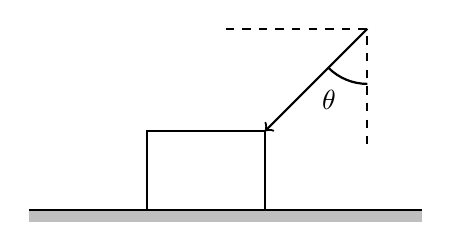
\begin{tikzpicture}
        \fill[gray!50](0,-.15) rectangle(5,0);
        \draw[thick](0,0)--(5,0);
        \draw[thick](1.5,0)rectangle(3,1);
        \draw[<-,thick](3,1)--(4.3,2.3);
          \draw[thick,dashed](2.5,2.3)--(4.3,2.3)--(4.3,.8);
          \draw[thick](4.3,1.6) arc(270:225:.7)
          node[midway,below left]{$\theta$};
      \end{tikzpicture}
    \end{center}
    \begin{choices}
      \choice $Fx\sin\theta$
      \choice $Fx\cos\theta$
      \choice $Fmx\sin\theta$
      \choice $Fmx\cos\theta$
      \choice zero
    \end{choices}
    
    \uplevel{
      \textbf{Questions \ref{sphere1}--\ref{sphere2}}\\
      A small block rests on the top of a smooth sphere of radius $R$ when it
      is given a light tap so that it just begins sliding on the sphere. When
      the block reaches the angle $\theta$, it loses contact with the surface
      of the sphere.
      \begin{center}
        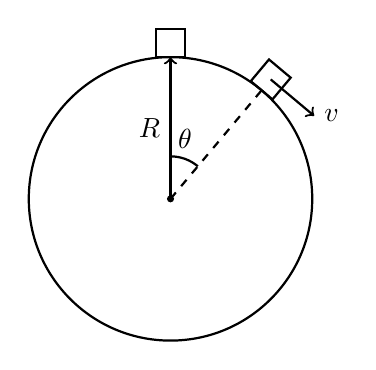
\begin{tikzpicture}[scale=.9]
          \draw[thick](0,0) circle(2);
          \fill(0,0) circle(.05);
          \draw[thick,->](0,0)--(0,2) node[midway,left]{$R$};
          \draw[thick](-.2,2) rectangle(.2,2.4);
          \begin{scope}[rotate around={-40:(0,0)}]
            \draw[thick,dashed](0,0)--(0,2);
            \draw[thick](-.2,2) rectangle(.2,2.4);
            \draw[->,thick](0,2.2)--(.8,2.2) node[right]{$\mb{v}$};
          \end{scope}
          \draw[thick](0,.6) arc(90:50:.6) node[midway,above]{$\theta$};
        \end{tikzpicture}
      \end{center}
    }

    \question The kinetic energy of the block as it leaves the surface of the
    sphere is
    \label{sphere1}
    \begin{choices}
      \choice $mgR$
      \choice $mgR\cos\theta$
      \choice $mgR\sin\theta$
      \choice $mg(R-R\cos\theta)$
      \choice $mg(R-R\sin\theta)$
    \end{choices}

    \question The speed of the block as it leaves the surface of the sphere is
    \label{sphere2}
    \begin{choices}
      \choice $\displaystyle\sqrt{2g}{m}$
      \choice $\displaystyle\sqrt{2gR}{m}$
      \choice $\displaystyle\sqrt{2gR\cos\theta}$
      \choice $\displaystyle\sqrt{2g(R-R\cos\theta)}$
      \choice $\displaystyle\sqrt{2g(R-R\sin\theta)}$
    \end{choices}
    
  \item A machine can lift large weights according to the power equation
    $P(t)=4t^3+3t^2-2$, where power is in watts and time is in seconds. The
    energy expended by the machine from $t=0$ to $t=\SI{10}{\second}$ is
    \begin{choices}
      \choice \SI{1260}{\joule}
      \choice \SI{3630}{\joule}
      \choice \SI{9240}{\joule}
      \choice \SI{10980}{\joule}
      \choice \SI{18150}{\joule}
    \end{choices}
    
    \question A small ball starts from rest and rolls down a quarter-circle
    ramp of radius $R$. The speed of the ball at the point halfway down the
    ramp is most nearly
    \begin{center}
      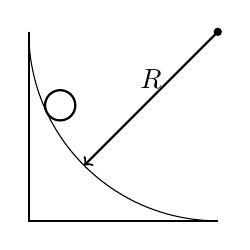
\begin{tikzpicture}[scale=2.4]
        \draw[thick](-1,0)--(-1,-1)--(0,-1);
        \draw(-1,0) arc(180:270:1);
        \draw[thick,->,rotate=45](0,0)--(-1,0) node[midway,above,sloped]{$R$};
        \draw[thick,rotate=25](-.92,0) circle(.08);
        \fill (0,0) circle(.022);
      \end{tikzpicture}
    \end{center}
    \begin{choices}
      \choice $gR$
      \choice $2gR$
      \choice $\displaystyle\sqrt{gR\sin\ang{45}}$
      \choice $\displaystyle\sqrt{2gR\sin\ang{45}}$
      \choice The speed cannot be determined without knowing the mass of the
      ball.
    \end{choices}
  \end{questions}
\end{multicols*}
\newpage

\genfreetitle{C}{WORK AND ENERGY}{4}

\genfreedirections

\begin{questions}

  \question A mass $m$ is placed on an incline of angle $\theta$ at a distance
  $d$ from the end of a spring as shown below. The coefficient of kinetic
  friction between the mass and the plane is $\mu$.
  \cpic{.3}{ramp1}
  \begin{parts}
    \part The mass is released from rest at the position shown. Using Newton's
    laws, calculate the block's speed when it reaches the spring.
    
    \part Using energy conservation, alculate the block's speed when it reaches
    the spring.
    
  \part The spring has spring constant $k$. At what value $x$ of the compression
    of the spring does the object reach its maximum speed?
  \end{parts}
  \newpage
  
e  % TAKEN FROM THE 2009 AP PHYSICS C EXAM FREE-RESPONSE QUETION MECH 1
  \question A \SI{3.}{\kilo\gram} object is moving along the $x$-axis in a
  region where its potential energy as a function of $x$ is given as
  $U(x)=4.0x^2$, where $U$ is in joules and $x$ is in meters. When the object
  passes the point $x=\SI{-0.50}{\metre}$, its velocity is
  $+$\SI{2.}{\metre\per\second}. All forces acting on the object are
  conservative.
  \begin{parts}
    \part Calculate the total mechanical energy of the object.
    
    \part Calculate the $x$-coordinate of any points at which the object has
    zero kinetic energy.
    
    \part Calculate the magnitude of the momentum of the object at
    $x=\SI{.60}{\metre}$.

    \part Calculate the magnitude of the acceleration of the object as it passes
    $x=\SI{.60}{\metre}$.
    
    \part On the axes below, sketch graphs of the object's position $x$ versus
    time $t$ and kinetic energy $K$ versus time $t$. Assume that $x=0$ at time
    $t=0$. The two graphs should cover the same time interval and use the same
    scale on the horizontal axes.
    \begin{center}
      \begin{tikzpicture}
        \draw[very thick,->](-1,0)--(10,0)node[right]{$t$};
        \draw[very thick,->](0,-3)--(0,3)node[above]{$x$};
      \end{tikzpicture}
      \vspace{.2in}
      \begin{tikzpicture}
        \draw[very thick,->](-1,0)--(10,0)node[right]{$t$};
        \draw[very thick,->](0,-3)--(0,3)node[above]{$K$};
      \end{tikzpicture}
    \end{center}
  \end{parts}
  \newpage
  
  % TAKEN FROM THE 2007 AP PHYSICS C MECHANICS FREE-RESPONSE QUESTION MECH 3
  \uplevel{
    \cpic{.7}{track1}
  }
  \question The apparatus above is used to study conservation of mechanical
  energy. A spring of force constant \SI{40}{\newton\per\metre} is held
  horizontal over a horizontal air track, with one end attached to the air
  track. A light string is attached to the other end of the spring and connects
  it to a glider of mass $m$. The glider is pulled to stretch the spring an
  amount $x$ from equilibrium and then released. Before reaching the photogate,
  the glider attains its maximum speed and the string becomes slack. The
  photogate measures the time t that it takes the small block on top of the
  glider to pass through. Information about the distance $x$ and the speed
  $\varv$ of the glider as it passes through the photogate are given below.
  \begin{center}
    \begin{tabular}{|c|c|c|c|c|}
      \hline
      Trial \#  & Extension of the Spring $x$ (m) &
      Speed of Glider &
      Extension Squared &
      Speed Squared \\
      & $x$ (\si{\metre}) & $\varv$ (\si{\metre\per\second}) &
      $x^2$ (\si{\metre\squared}) & $\varv^2$ (\si{m^2/s^2}) \\
      \hline
      1 & \num{0.30e-1} & 0.47 & \num{0.09e-2} & 0.22\\\hline
      2 & \num{0.60e-1} & 0.87 & \num{0.36e-2} & 0.76\\\hline
      3 & \num{0.90e-1} & 1.3  & \num{0.81e-2} & 1.7\\\hline
      4 & \num{1.2 e-1} & 1.6  & \num{1.4 e-2} & 2.6\\\hline
      5 & \num{1.5 e-1} & 2.2  & \num{2.3 e-2} & 4.8\\\hline
    \end{tabular}
  \end{center}
  \begin{parts}
    \part Assuming no energy is lost, write the equation for conservation of
    mechanical energy that would apply to this situation.
    
    \part On the grid below, plot $\varv^2$ versus $x^2$. Label the axes,
    including units and scale.

    \vspace{.1in}
    \begin{center}
      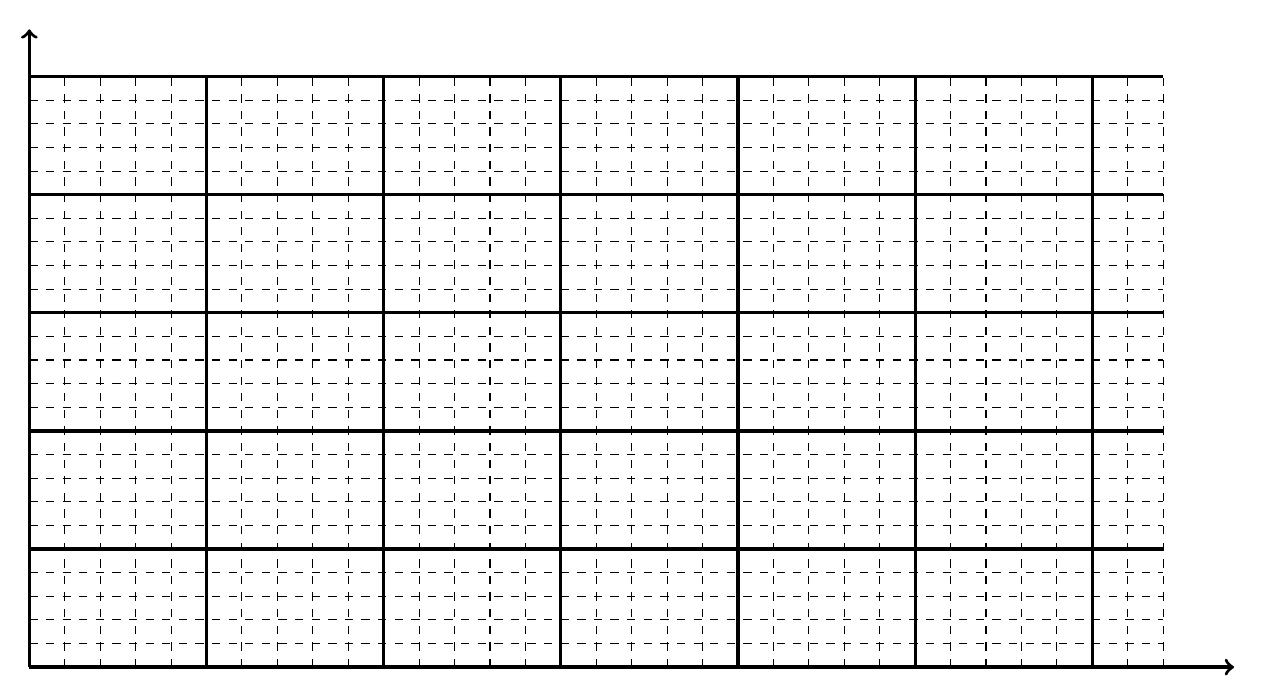
\begin{tikzpicture}[yscale=.3,xscale=.45]
        \draw[very thick,->](0,0)--(34,0);
        \draw[very thick,->](0,0)--(0,27);
        \draw[dashed](0,0) grid(32,25);
        \draw[very thick,step=5](0,0) grid(32,25);
      \end{tikzpicture}
    \end{center}

    \part
    \begin{subparts}
      \subpart Draw a best-fit straight line through the data.
      \subpart Use the best-fit line to obtain the mass $m$ of the glider.
    \end{subparts}
    
    \part The track is now tilted at an angle $\theta$ as shown below. When the
    spring is unstretched, the center of the glider is a height $h$ above the
    photogate. The experiment is repeated with a variety of values of $x$.
    \cpic{.7}{track2}
    
    \begin{subparts}
      \subpart Assuming no energy is lost, write the new equation for
      conservation of mechanical energy that would apply to this situation.
      
      \subpart Will the graph of $\varv^2$ versus $x^2$ for this new experiment
      be a straight line? Justify your answer.

      \vspace{.1in}
      \underline{\hspace{.5in}} Yes\hspace{.5in}
      \underline{\hspace{.5in}} No
    \end{subparts}
  \end{parts}
  \newpage

  % TAKEN FROM 2012 AP PHYSICS C MECHANICS EXAM FREE-RESPONSE QUESTION MECH 2
  \question You are to perform an experiment investigating the conservation of
  mechanical energy involving a transformation from initial gravitational
  potential energy to translational kinetic energy.
  \begin{parts}
    \part You are given the equipment listed below, all the supports required
    to hold the equipment, and a lab table. On the list below, indicate each
    piece of equipment you would use by checking the line next to each item.

    \begin{tabular}{lll}
      \underline{\hspace{.3in}} Track &
      \underline{\hspace{.3in}} Meterstick &
      \underline{\hspace{.3in}} Set of objects of different masses\\
      \underline{\hspace{.3in}} Cart &
      \underline{\hspace{.3in}} Electronic balance &
      \underline{\hspace{.3in}} Lightweight low-friction pulley\\
      \underline{\hspace{.3in}} String &
      \underline{\hspace{.3in}} Stopwatch & \\
    \end{tabular}

    \part Outline a procedure for performing the experiment. Include a diagram
    of your experimental setup. Label the equipment in your diagram. Also
    include a description of the measurements you would make and a symbol for
    each measurement.
    \label{procedure}
    
    \part Give a detailed account of the calculations of gravitational
    potential energy and translational kinetic energy both before and after the
    transformation, in terms of the quantities measured in part
    (\ref{procedure}).

    \part After your first trial, your calculations show that the energy
    increased during the experiment. Assuming you made no mathematical errors,
    give a reasonable explanation for this result.

    \part On all other trials, your calculations show that the energy decreased
    during the experiment. Assuming you made no mathematical errors, give a
    reasonable physical explanation for the fact that the average energy you
    determined decreased. Include references to conservative and
    nonconservative forces, as appropriate.
  \end{parts}
  
%\item The theoretical formula for the potential energy associated with the
%  nuclear force between two protons, two neutrons, or a proton and a neutron
%  is the \emph{Yukawa potential}:
%  \begin{displaymath}
%    U=-U_0\left(\frac{a}{x}\right)e^{-x/a}
%  \end{displaymath}
%  where $U_0$ and $a$ are constants.
%  \begin{enumerate}[noitemsep]
%  \item Sketch $U$ versus $x$ using $U_0=\SI{4}{\pico\joule}$ and
%    $a=\SI{2.5}{\femto\metre}$.
%  \item Find the force $F_x$.
%  \item Compare the magnitude of the force at the separation $x=2a$ to that at
%    $x=a$.
%  \item Compare the magnitude of the force at the separation $x=5a$ to that at
%    $x=a$.
%  \end{enumerate}
%  \vspace{\stretch{1}}
%  \newpage
  
%\item A small block of mass $m$ slides without friction along the loop-the-loop
%  track shown in the figure. The block starts from point $P$ a distance $h$
%  above the bottom of the loop.
%  \begin{center}
%    \begin{tikzpicture}[scale=1.2]
%      \fill[blue!30!black](0,0) circle(1);
%      \fill[white](0,0) circle(.88);
%      \fill(0,0) circle(.05);
%      \draw[thick,->](0,0)--(.88,0)node[midway,above]{\scriptsize$R$};
%      \draw[dashed](-4,-1)--(2,-1);
%      \fill[rotate=15,blue!30!black](0,-1)rectangle(2,-.88);
%        \begin{scope}[rotate=-45]
%          \fill[blue!30!black](0,-1)rectangle(-4,-.88);
%          \fill[blue](-3,-.88)rectangle(-3.3,-.58)
%          node[black,right]{\scriptsize$m$};
%        \end{scope}
%        \draw[<->](-3,-1)--(-3,1.5) node[midway,left]{\scriptsize$h$};
%        \draw(-2.9,1.5)--(-3.1,1.5) node[left]{\scriptsize$P$};
%    \end{tikzpicture}
%  \end{center}
%  \begin{enumerate}[nosep]
%  \item What is the kinetic energy of the block when it reaches the top of
%    the loop?
%  \item What is the acceleration at the top of the loop, assuming that it
%    stays on the track?
%  \item What is the least value of $h$ for which the block will reach the top
%    of the loop without leaving the track?
%  \end{enumerate}
%  \newpage
%
%\item A pendulum of length $L$ has a bob of mass $m$. It is released from some
%  angle $\theta_1$. The string hits a peg at a distance $x$ directly below the
%  pivot, as shown in the figure below, effectively shortening the length of the
%  pendulum. Find the maximum angle $\theta_2$ between the string and the
%  vertical when the bob is to the right of the peg.
%  \begin{center}
%    \pic{.4}{pendulum-peg}
%  \end{center}
%  \vspace{\stretch1}
%  \newpage
%  
%\item A \SI{2.}{\kilo\gram} block $m$ is released \SI{4.}{\metre} from a
%  massless
%  spring with a spring constant of $k=\SI{100}{\newton\per\metre}$ that is fixed
%  along a frictionless plane inclined at \ang{30}, as shown in the figure below.
%  (Plese give answer to $3$ significant figures.)
%  \begin{center}
%    \begin{tikzpicture}[scale=.7]
%      \begin{scope}[rotate=-30]
%        \fill(0,0) rectangle(-.1,1);
%        \draw[thick,
%          decoration={aspect=.4,segment length=1.5mm, amplitude=2mm,coil},
%          decorate] (-.1,.5)--(-1.5,.5)
%        node[midway,above right]{$k$};
%        \fill(-1.5,0) rectangle(-1.6,1);
%        \draw[<->,thick](-1.6,1.5)--(-5.6,1.5)
%        node[midway,above right,sloped]{\SI{4.}{\metre}};
%        \draw[thick](-1.6,1.05)--(-1.6,2);
%        \draw[thick](-5.6,1.05)--(-5.6,2);
%        \draw[fill=yellow!50](-5.6,0) rectangle(-6.3,.7)
%        node[black,above left]{$m$};
%      \end{scope}
%      \draw[fill=pink!50](0,0)--(-6.06,0)--(-6.06,3.5)--cycle;
%      \draw[<->,thick](-2,0) arc(180:150:2) node[midway,left]{\ang{30}};
%    \end{tikzpicture}
%  \end{center}
%  \begin{enumerate}[noitemsep,leftmargin=20pt]
%  \item Find the maximum compression of the spring.
%  \item If the plane is not frictionless, and the coefficient of kinetic
%    friction between it and the block is $\mu=0.20$, find the maximum
%    compression.
%  \item For the rough incline ($\mu=0.20$), how far up the incline will the
%    block travel after leaving the spring?
%  \end{enumerate}
\end{questions}
\end{document}
